\documentclass[%
 aip,
cp,  
 amsmath,amssymb,
 reprint,
]{iopconfser}

\usepackage{graphicx}% Include figure files
\usepackage{dcolumn}% Align table columns on decimal point
\usepackage{bm}% bold math
%\usepackage[mathlines]{lineno}% Enable numbering of text and display math
%\linenumbers\relax % Commence numbering lines

\usepackage[utf8]{inputenc}
\usepackage[T1]{fontenc}
%% Loads a Times-like font. You can also load
%% {newtxtext,newtxtmath}, but not {times}, 
%% {txfonts} nor {mathtpm} as these packages
%% are obsolete and have been known to cause problems.
\usepackage{mathptmx} 
\usepackage{multirow}
\usepackage{float}
\usepackage{amsmath}
\usepackage{amsfonts}
  
\newcommand{\be}{\begin{equation}}
\newcommand{\ee}{\end{equation}}
\newcommand{\rf}[1]{(\ref{#1})}
\newcommand{\RR}{\mathbb{R}}
\newtheorem{thm}{Theorem}
\newtheorem{lm}{Lemma}

\begin{document}

\title{Numerical Study of the good Boussinesq Equation}

\author{Krassimir Angelow$^{1}$ and Veselina Vucheva$^{2}$}

\affil{$^{1}$  $^{2}$Institute of Mathematics and Informatics, Bulgarian Academy of Sciences, Acad., \\ G.~Bonchev Bl.8, 1113, Sofia, Bulgaria}


\email{angelow@math.bas.bg}

\begin{abstract}
In this paper we evaluate propagating wave solutions to the one-dimensional good Boussinesq Equation (BE).
Two numerical methods are used to obtain a solution. The first is a conservative finite difference scheme, and the second exploits Taylor series expansions around the time variable $t$. 
The solutions are computed over nested meshes to examine the convergence of both approaches. The main tool for testing the convergence rate of all examined finite difference schemes and Taylor expansions is the Runge's method. It is shown that for a fixed time interval the numerical methods preserve the shape of the waves after interaction and mass of the solution. The waves obtained by the two methods are compared with the exact solution.
Both methods produce similar results in case of $O(h^{2} + \tau^2 )$ approximation order, with errors measured in $L_2$ and $L_\infty$ norms which are 100 times or less than the solution maximum.
\end{abstract}

\section{\label{sec:level1}Introduction}

The Boussinesq type equations are famous with the approximation of shallow water waves or also weakly non--linear long waves. It is often used for simulation of various physical processes e.g. turbulence in fluid mechanics, vibrations in acoustics, etc. For the numerical interaction of Boussinesq traveling waves (TW) one needs the shape of a stationary wave in order to build the Initial Condition (IC) $u_0$, $u_1$.

The shallow water model developed by Boussinesq and the equaitons he derived in this conjuction were first described in \cite{ref0}. The equation is known to have an explicit solution in the case of one moving solitary wave. It is also known that it has a solution with two solitary waves that results in their temporary combination and subsequent reemergence in their original forms after the interaction \cite{exactSol1, exactSol2}. An improvement of the Boussinesq model was done by Christov's "energy-consistent approximation" \cite{ref1} a.k.a the Boussinesq Paradigm Equation (BPE). Christov states that the original model with the initial value problem defined by Boussinesq is incorect in the sense of Hadamard (see \cite{ref1}), i.e. even small perturbations in the initial or boundary conditions could lead to significant differences in the behavior of the solution over time. Unfortunately the BPE is not known to posses an explicit solution in the case of two solitary waves. We would like to compare the numerical and the exact solutions in the case of two solitary waves. This could be done in the case of the original (a.k.a good) Boussinesq model:
\begin{align}\label{orgBsq}
&\frac{\partial^2 }{\partial t^2}u(x,t)= \frac{\partial^2}{\partial x^2}u(x,t) -  \frac{\partial^4}{\partial x^4}u(x,t) - 3\frac{\partial^2}{\partial x^2} f(u(x,t))
\\
&u(x,0) = u_0(x), \quad \frac{\partial }{\partial t}u(x,0)=u_1(x), \nonumber
\\
&u(x,t) \rightarrow 0, \quad \frac{\partial }{\partial t} u(x, t) \rightarrow 0 \quad \text{for} \quad |x| \rightarrow \infty, \nonumber
\end{align}
where $f(u) = u^2$. The domain of the unknown function $u$ is defined by:
\be
 u:\Omega \times [0, T] \rightarrow \RR,
\ee
where $\Omega \equiv (-\infty, \infty)$ and $T>0$. The continuous energy of the solution is defined by
\begin{eqnarray}\label{con-cont2}
E\left( u(x,t)\right)=	\frac{1}{2} \left\|(-\partial^2_x)^{-1/2} \frac{\partial u}{\partial t}(x,t)\right\|^2 + \frac{1}{2}  \left\|u (x,t)\right\|^2 
+ \frac{1}{2}\left\| \nabla u(x,t) \right\|^2+ \int _{R} u(x,t)^3 dx.
\end{eqnarray}
The mass of the solution is defined by
\begin{equation}\label{intM}
M(u(x,t))=\int_{\RR} u(x,t)dx,
\end{equation}
Equation \rf{orgBsq} is equivalent to the BPE if the mixed time and space derivative is omited. E.g. if we set $\beta_1 = 0$, $\beta_2 = 1$ and $\alpha = 3$ in equation (2) from article \cite{ref21} (Chertock, Christov, Kurganov) then it is equivalent to \rf{orgBsq} defined above. Equation \rf{orgBsq} obtains two wave soliton solution (see formula \rf{orgBsqSol} defined in section Numerical Results).
The soliton is localized wave, which moves at constant velocity ($\omega_i, \: i=1,2$ in case of \rf{orgBsqSol}) and maintains its shape. When a soliton interacts with another soliton, it emerges from the "collision" unchanged, i.e. its amplitude, shape, and velocity are conserved. 

The goal of the article is to show that one could obtain a numerical solution for the 1D problem \rf{orgBsq} in the frame of two solitary waves moving towards each other. Furthermore, the numerical analysis shows that increasing the approximation order and decreasing the space step, produces  numerical solution with smaller error norms. The mass and the energy (in case of the Conservative Finite Difference Scheme) norms are preserved with the same accuracy as the numerical solution. The results and observations for the good Boussinesq equation \rf{orgBsq} could be further used in order to find a two wave solitary solution for the 1D and 2D BPE.

The paper is organized as follows. Section 2 introduces the numerical methods that are used for equation \rf{orgBsq}: Method with Conservative Finite Difference Scheme (FDS) and Taylor method, which uses Taylor Series (TS) expansions around the time variable $t$. Section 3 concerns the numerical results. It states the initial condition, boundary condition, space and time domains. The numerical calculations are done over nested meshes to examine the convergence of both methods. The goal is to justify the TS approach by showing that both methods exhibit similar results. Furthermore the TS method could be used with higher approximation order which produces a finer solution. Subsection 3.1 shows the convergence speed of the Conservative FDS and energy measured with Rugne's rule. The next section shows the convergence speed of the Taylor method. Furthermore, for each method, the mass of the solution is calculated which is described in Subsection 3.3. In Subsection 3.4, the shape of the numerical solution, obtained from both methods, is compared against the exact solution. In Subsection 3.5, the shape, mass and energy of the solution are investigated one more time, over a larger time interval, where the solitary waves pass through each other. The last section gives an overview of the achieved goals and summarize the results.

\section{Numerical Methods}

The space domain $(-\infty,\infty)$ is replaced with a finite  interval $[L_1,L_2]$, where $|L_i|$, $i=1,2$ are sufficiently large numbers, so that the exact solution to \rf{orgBsq} and its derivatives are negligible outside this interval. A uniform grid $x_i$,  $i=0,1,\cdots N$ is introduced with step $h=|L_2-L_1|/(N-1)$ in the interval $[L_1,L_2]$. The space domain is one dimensional, and the $\Delta_h$ operator below denotes the approximation of the second derivative $\partial^2/\partial x^2$.
Let $\tau$ be the time step in $[T_0,T]$ and $T=T_0+K \tau$ be the final time. 

\subsection{ Conservative Finite Difference Scheme with weight $\sigma$ and approximation error $O(h^2+\tau^2)$}

We use the following finite differences
\begin{equation}\label{secDerfd}
y_{\bar{t}t,i}^k=\dfrac{y_i^{k+1}-2y_i^k+y_i^{k-1}}{\tau^2},~~\Delta_h y_i^k=\dfrac{y_{i+1}^k-2y_i^k+y_{i-1}^k}{h^2}
\end{equation}
\begin{equation}\label{forDerfd}
\Delta_h^2 y_i^k=\dfrac{y_{i+2}^k-4y_{i+1}^k+6y_{i}^k-4y_{i-1}^k+y_{i-2}^k}{h^4}.
\end{equation}
Here $y_{i}^k$ denotes the approximation of the unknown function $u$, on node $x_i$, at moment $t_k = T_0 + k \tau$, i.e. $y_{i}^k \approx u(x_i,t_k)$. Replacing the derivatives \rf{secDerfd} and \rf{forDerfd} in \rf{orgBsq} leads to the following equation:
\begin{equation}\label{scheme1}
y_{\bar{t}t,i}^k=\Delta_h y_i^{\sigma,k}-\Delta_h^2 y_i^{\sigma,k} - 3\Delta_h g(y_i^k).
\end{equation}
Here $ y_i^{\sigma,k}= y_i^{k}+\sigma \tau^2 y_{\bar{t}t,i}^k$ and the nonlinear term is approximated as in \cite{consCitat} with:
\begin{equation}\label{nonLin}
g(y_i^k) = \frac{1}{3} \frac{(y_i^{k+1})^3 - (y_i^{k-1})^3}{y_i^{k+1} - y_i^{k-1}}.
\end{equation}

This leads to the following Conservative finite difference scheme:
\begin{eqnarray}\label{mainConsScheme}
\dfrac{\sigma\tau^2}{h^4}y_{i-2}^{k+1}+\left(-4\dfrac{\sigma\tau^2}{h^4}-\dfrac{\sigma\tau^2}{h^2}\right)y_{i-1}^{k+1}+\left(1+6\dfrac{\sigma\tau^2}{h^4}+2\dfrac{\sigma\tau^2}{h^2}\right)y_{i}^{k+1}+\left(-4\dfrac{\sigma\tau^2}{h^4}-\dfrac{\sigma\tau^2}{h^2}\right)y_{i+1}^{k+1}+\dfrac{\sigma\tau^2}{h^4}y_{i+2}^{k+1}=\nonumber\\
=2y_i^k-y_i^{k-1}-2\sigma\tau^2\Delta_h y_i^k+\sigma\tau^2\Delta_hy_i^{k-1}+2\sigma\tau^2\Delta_h^2y_i^k-\sigma\tau^2\Delta_h^2y_i^{k-1}+\tau^2\left(\Delta_hy_i^k-\Delta_h^2y_i^k-3\Delta_h g(y_i^k)\right).
\end{eqnarray}

The last equation needs to be resolved for the upper time layer $y^{k+1}$ and the nonlinear term also depends on $y^{k+1}$, which makes \rf{mainConsScheme} implicit. For this, we do Piccard iterations at each time step.

The complexity of the Conservative FDS applied for the Good Boussinesq equation is
$$ O( N_x  N_t ) $$
where $N_x$ is the number of points in $\Omega_h$ and $N_t = T/\tau$. The most time consumable operation is inverting the following five band matrix 

$$\left[ \dfrac{\sigma\tau^2}{h^4}, \left(-4\dfrac{\sigma\tau^2}{h^4}-\dfrac{\sigma\tau^2}{h^2}\right), \left(1+6\dfrac{\sigma\tau^2}{h^4}+2\dfrac{\sigma\tau^2}{h^2}\right), \left(-4\dfrac{\sigma\tau^2}{h^4}-\dfrac{\sigma\tau^2}{h^2}\right), \dfrac{\sigma\tau^2}{h^4} \right]$$

which results from equation \rf{mainConsScheme}. This is an operation with $ O( N_x ) $ algorithmic complexity. The use of Picard iterations (which are not more than six per time step) affects complexity by a constant.
\subsection{Discrete energy}

Let $E_h (y^k)$ be the discrete energy, which is defined in the following way:
\begin{eqnarray}\label{energy1}
E_h (y^k):=E_{h,L} (y^k) +\frac{1}{2}((y^{k+1})^3+(y^{k})^3,1).
\end{eqnarray}
The linear part $E_{h,L}$ is given by
\begin{align*}\label{den}
E_{h,L}\left( y^k \right)&:= 
\dfrac{1}{2}\left(A^{-1/2}y_t^k,A^{-1/2}y_t^k\right)+\left(\dfrac{\sigma\tau^2}{2}-\dfrac{\tau^2}{8}\right)\left(y_t^k,y_t^k\right)+\nonumber\\&+\left(\dfrac{\sigma\tau^2}{2}-\dfrac{\tau^2}{8}\right) \left(Ay_t^k,y_t^k\right)
+\dfrac{1}{8}\left(\left(I_d+A\right)\left(y^{k+1}+y^k\right),y^{k+1}+y^k\right)
\end{align*}

where $A=-\Delta_h$ and $I_d$ is the Identity matrix. The discrete energy $E_h (y^k)$ approximates the energy \rf{con-cont2} with error $O(h^2+\tau^2)$.


{\textbf{Discrete conservation law}}
%	The finite difference scheme \rf{scheme1} is conservative, i.e. the discrete energy $E_h(y^k)$, given by с \rf{energy1}, is preserved in time: 
	$$E_h(y^k)=E_h(y^0),~k=1,2,...,K.$$

The proof is a consequence of the stability results from the book of Samarskii \cite{samarski} and it is derived in \cite{consCitat}.

\subsection{ Taylor Series Approach with Method of Lines}
Here we proceed as in \cite{refHyp} and use similar approach as the one defined for the BPE.
The finite differences along space and time discretization require Taylor Series (TS) expansions of $u(x,t)$. Therefore it is assumed that the solution is $p+1$ times infinitely differentiable with respect to $x$ and $t$, i.e. $u \in C^{p+1,p+1}(\Omega \times T)$.
For the Taylor method two different approximations of the spatial differential operator $\Delta_h$ are used. The following central finite differences along the $x$ asis are applied:
\begin{equation}\label{fd}
u_{\widehat{xx},p}(x,y) :=  \Delta_h u  = \frac{1}{h^2} \sum\limits_{i=-p/2}^{p/2} d_i u(x+ih, t).
\end{equation}
The weights $d_i$ are defined below in Table \rf{table:A00}.
\begin{table}[ht]
\centering
\small
		\begin{tabular}{|c|l|l|l|l|l|}

			\hline
            $p=2$          &                                           &     1      &   -2   &    1       &     \\
   			\hline 
           $p=4$          &                              $-\frac{1}{12}$     &     $\frac{4}{3}$      &   $-\frac{5}{2} $     &    $\frac{4}{3}$    &  $-\frac{1}{12}$      \\ 
	   \hline
		\end{tabular}
	\caption{ Finite differences used for the approximation of the Laplace operator.}
	\label{table:A00}
\end{table}
E.g. if $p=2$, then \rf{fd} is equivalent to the spatial finite difference in \rf{secDerfd}.  The approximation error of formulas \rf{fd} is $O(h^p)$. Let $u_{i}(t)$ and $u_{i, \widehat{xx}, p}(t)$ be the approximations of the unknown function $u$ and its second derivative $u_{xx}$ at arbitrary mesh point $(x_i)$ for arbitrary time $t$. Then one obtains a system of ODEs:
\be \label{DiscreteEq}
\frac{\partial^2 }{\partial t^2}u(x_i, t) =
(u_{i} - u_{i, \widehat{xx}, p} - 3u^2_{i})_{\widehat{xx}, p}(t) 
\ee
for all mesh points $i = 0..N_x$. For each ODE in the system we do TS expansion along the time variable:
\begin{align} \label{TSe}
u(x_i, t+\tau) = u(x_i, t) + \tau \frac{ \partial u }{ \partial t }(x_i,t)  + ... 
%\nonumber
%\\
\frac{ \tau^p }{ p! } \frac{ \partial^p u }{ \partial t^p }(x_i, t) + O(\tau^{p+1})
\end{align}
for some natural number $p \ge 2$. The approximation order of the time discretization depends on p, i.e. the number of terms included in the TS expansion. Each point on the mesh represents a starting point of a line and the line itself is described by the TS expansion \rf{TSe}. Evaluation of formula \rf{TSe} is done by evaluating each term separately. E.g. for $t=0$ the first two terms are known from the IC ($u_0$, $u_1$). The third term is evaluated from the discrete equation \rf{DiscreteEq}. With subsequent differentiaton of equation \rf{DiscreteEq} one could obtain higher time derivatives $\frac{\partial^3 u}{\partial t^3}$, $\frac{\partial^4 u}{\partial t^4}$, etc. This is an iterative procedure where e.g. the fourth time derivative requires 2nd, 1st and 0th derivatives, 3rd time derivative requires 1st and 0th derivatives. After all necessary time derivatives are calculated one could substitute those in \rf{TSe} and gets the following approximations: for $p=2$ it is $O(|h|^2 + \tau^2)$ and for $p=4$ it is $O(|h|^4 + \tau^4)$. Note that another TS expansion must be calculated for the first time derivative $u_t(x_i, t+\tau)$, which is analogous to \rf{TSe} with the same approximation order. The last is required in order to calculate the solution on the next time layer because the pair ($u$, $u_t$) serve as basis and all higher time derivatives could be expressed only by that pair.

The complexity of the algorithm is
$$ O( N_x  N_t ) $$
where $N_x$ is the number of points in $\Omega_h$ and $N_t = T/\tau$. Current choices of $p$ affect complexity by a constant which resutls in a linear time graph depending on the number of points in the discrete domain.


\section{Numerical Results}

The convergence rates for the Conservative FDS and Taylor method are calculated. At the end, the properties of the solution that are obtained numerically by the two different mechanisms are compared. The mass is a vector of size $N_t$ and is calculated for each iteration step. The tool for testing the convergence rate $\xi$ of all examined finite difference schemes and TS expansions is the Runge's method
\begin{equation}\label{Runge}
\xi = ln  \frac{\Vert u_{h} - (u_{ex})_{h} \Vert_\kappa } {\Vert  u_{h/2} - (u_{ex})_{h/2} \Vert_\kappa  } | / ln(2),
\end{equation}
where $u_{ex}$ is the exact solution \rf{orgBsqSol}, which is defined below, over the corresponding grid with step size $h$ or $h/2$. Here, $\kappa$ denotes the used norm, which is either $L_2$ or $L_\infty$. The time step $\tau$ is kept constant.
\begin{align}\label{orgBsqSol}
u(x,t) =& -2 \frac{\partial ln F(x,t)}{\partial x^2},
\\
 F(x,t) =& a_0 + a_1 e^{k_1 x + \omega_1 t + b_1} + a_2 e^{k_2 x + \omega_2 t + b_2}  + a_{12} e^{(k_1 + k_2) x + (\omega_1 + \omega_2)  t + b_1 + b_2}, \nonumber
\\
|k_i| <& 1, \; \omega_i = \sqrt{k^2_i(1-k^2_i) }, \; k_i \neq 0, \quad i = 1,2, \nonumber
\\
a_0 =& \frac{a_1 a_2}{a_{12}}\frac{4k_1^4 + 4k_2^4 - 3k_1^2 - 3k_2^2 - 2k_1^2 k_2^2 + 6\sqrt{k_1^2-k_1^4}\sqrt{k_2^2-k_2^4} }{(k_1 + k_2)^2 (4(k_1^2 + k_1 k_2 + k_2^2) - 3)}.\nonumber
\end{align}
Most of the work for the derivation of the exact solution, with two solitary waves, could be found in \cite{exactSol1, exactSol2}. Some additional calculations were done by Vasil Vasilev where he provided formulas \rf{orgBsqSol} (private communication). 
The parameters in \rf{orgBsqSol} for the numerical tests are defined as:
\be\label{params}
        k_1 = 1/3,  \;\; k_2 = -1/2,  \;\; b_1 = -20\sqrt{(k_1^ 2  (1 - k_1 ^ 2))}, \;\; b_2 = -20\sqrt{(k_2^ 2  (1 - k_2^2))},  \;\; a_1 = a_2 = a_{12} = 1.
\ee
The exact solution, with the above parameters (see Figure \rf{ex_sol}), is tested against the differential equation \rf{orgBsq}, using free software mathematical applications, which justified the validity of \rf{orgBsqSol}.
\begin{figure}[ht]\vspace{0.2cm}
  \centering
  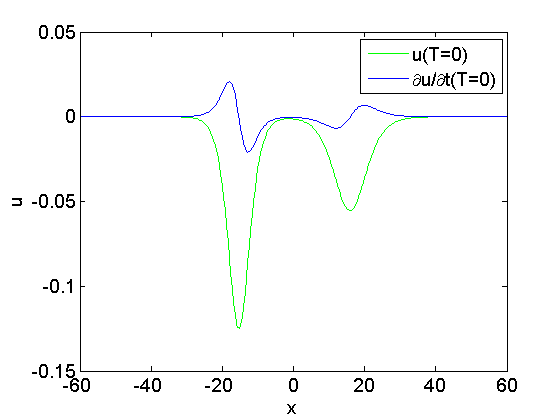
\includegraphics[width=0.5\linewidth]{IC.png}
\caption{The exact solution \rf{orgBsqSol} and its time derivative with parameters defined in \rf{params}. These are the two waves which move against each other. }
\label{ex_sol}
\end{figure}

The numerical tests for both, the Conservative FDS and Taylor method ($p=2$), show that the time step needs to be smaller than the space step squared $\tau < h^2 < 1$. For the Taylor method with $p=4$, the restriction is even stronger. Otherwise, the solution diverges and becomes non-smooth (e.g. the graph is jagged) and there is no convergence (see Figure \ref{figConvSeq}b)). The last explains the choice of $h, \tau$ when measuring the convergence speed in Table \rf{tableC}, Table \rf{tableD} and Table \rf{tableA}. A short numerical analysis on the this statement could be found in Subsection 3.2 and Figure \rf{figConvSeq}, where we measure the effect of decreasing the time step on the convergence speed. It is also inapplicable to measure the time convergence as the space errors are much higher ( $\tau < h^2 < 1$ ). Thus the time step $\tau$ is kept constant when measuring convergence speed with Runge's rule \rf{Runge}.

%0
\begin{table}[ht]
\centering
\small
		\begin{tabular}{|c|l|l|l|l|l|}
			\hline
                               &           Variant a  &           Variant b     &     \\
			\hline
            Grid 1          &            $h=0.4$  &            $h=0.2$     &    $\tau = 2.5e-04$  \\
			\hline
            %Grid 1a          &            $h=0.4$     &    $\tau = 2.5e-04$  \\
%			\hline
          %  Grid 1b          &            $h=0.2$     &    $\tau = 2.5e-04$  \\
   %			\hline 
           Grid 2         &            $h=0.4$  &   $h=0.2$  &    $\tau =1.0e-06$   \\   
   			\hline 
      %     Grid 2b         &            $h=0.2$  &    $\tau =1.0e-06$   \\    
%	   \hline
   %        Grid 3a          &            $h=0.8$  &    $\tau =6.25e-05$   \\    
%	   \hline
           Grid 3         &            $h=0.8$  &            $h=0.4$  &    $\tau =6.25e-05$   \\    
	   \hline
		\end{tabular}
	\caption{ Space and time steps used to benchmark the Conservative FDS and the Taylor method.}
	\label{gridsT}
\end{table}

The numerical methods described in the article are tested (at least) on six different grids defined in Table \rf{gridsT}. The Conservative FDS uses second approximation order on all grids while the Taylor method uses second approximation order on Grid 1 and fourth on Grid 2 and Grid 3. Later, other combinations of $h$ and $\tau$ are also used and are explicitly defined.

The discrete time interval for the numerical simulations is $[0, 10]$ unless stated otherwise. For that time, the two waves move against each other and at the moment $T=10$ are seen just before their collision. There is one additional experiment, with a time interval [0, 35], where the waves pass through each other (i.e. collide) and the distance between them at the final moment $T$ is approximately the same as at the initial moment $T_0$. 

All computations are done with $-L_1 = L_2 = 60$.
Zero boundary condition is used on the computational edges of the space domain $[L_1, L_2]$. In case of the second derivative, with fourth approximation order, used inside the Taylor method, the finite difference stencil extends an extra point outside the $L_1$ and $L_2$ boundaries and the numerical solution is approximated again with $0$. The same is also valid for the fourth spatial derivative, with second approximation order, used in the Conservative FDS. This decision is taken because, the unknown function near the computational boundaries is calculated to be lower than $1e-10$ (using \rf{orgBsqSol}). Furthermore, it is confirmed that
this approximation does not affect the convergence speed caclulated with Runge's rule (see Table \rf{tableA}).

\subsection{Convergence Rate for the Conservative FDS}

Table \ref{tableC} measures the convergence speed based on the results of the numerical solution $u_h$. The $\sigma$ parameter in \rf{mainConsScheme} is set to $\sigma = 0.75$. 
%C
\begin{table}[ht]
\centering
\small
		\begin{tabular}{||c|l|ll|ll||}
			\hline
			\hline
      \multirow{2  }{*}{FDS}        & \multirow{2  }{*}{$h$, $\tau$}  & \multirow{2  }{*}{errors $E_i$in$L_2$}  &Conv.& \multirow{2  }{*}{errors $E_i$in$L_\infty$}  &Conv.  \\
	                                        &                                                     &                                                                 &  Rate &                                                                       & Rate \\
   			\hline 
					\hline 
                                   &0.4, 0.001         & 0.0007711747   &                & 0.0005850814  &           \\
   $O(h^2 + \tau^ 2)$  &0.2, 0.001         & 0.0001231543   & 2.65       & 0.0001279704   &    2.19   \\
                                   &0.1, 0.001        & 0.0000193704    & 2.67     & 0.0000236392   &   2.44   \\
	   \hline
			\hline 
		\end{tabular}
		\caption{Space convergence speed for the solution obtained by the Conservative FDS with zero boundary conditions and approximation errors $O(h^{2})$. Errors $E_i$ are measured in $L_2$ and $L_\infty$ norms}
\label{tableC}
\end{table}
%D
\begin{table}[ht]
\centering
\small
		\begin{tabular}{||c|l|ll|ll||}
			\hline
			\hline
      \multirow{2  }{*}{FDS}        & \multirow{2  }{*}{$h$, $\tau$}  & \multirow{2  }{*}{errors $E_i$in$L_2$}  &Conv.& \multirow{2  }{*}{errors $E_i$in$L_\infty$}  &Conv.  \\
	                                        &                                                     &                                                                 &  Rate &                                                                       & Rate \\
   			\hline 
					\hline 
                                   &0.4, 0.001         &                    &                &                  &                   \\
                                   &0.2, 0.001        & 0.0000006687  &                & 0.0000149559   &                   \\
     $O(h^2 + \tau^ 2)$ &0.1, 0.001      & 0.0000001757   & 1.93       & 0.0000039284 & 1.93   \\
                                     &0.05, 0.001  & 0.0000000482   & 1.87       & 0.0000010792  & 1.86   \\
	   \hline
			\hline 
		\end{tabular}
		\caption{ Convergence speed for the discrete energy using the Conservative FDS and approximation errors $O(h^{2})$. Errors $E_i$ are measured in $L_2$ and $L_\infty$ norms. }
\label{tableD}
\end{table}
The Conservative FDS applies only second approximation order, thus $p=2$ for all completed tests in this subsection. Four nested meshes are used with different step sizes which are present in the second column. The next two columns show the errors $\Vert u_{h} - (u_{ex})_{h} \Vert_\kappa$, $\Vert  u_{(h/2)} - (u_{ex})_{h/2} \Vert_\kappa$ and convergence speed $\xi$ from \rf{Runge} which are measured in $L_2$ and infinity norms. The time step $\tau = 0.001$ is kept constant.

Table \ref{tableD} is analogous to Table \ref{tableC} and measures the convergence speed based on the results of the discrete energy \rf{energy1}. The convergence rate of both solution and energy is found to be in correspondence with the second spatial order approximation that is used.

The value of the initial energy is $0.0889$ and is computed using formula \rf{energy1}. The maximum deviation from the initial value equals $8.6644e-07$ for $h=0.4$, $8.6649e-07$ for $h=0.2$ and $8.6490e-07$ for $h=0.1$. Those differences are in correspondence with the errors $|E_i|_{L_2}$ and $|E_i|_{L_\infty}$ measured in Table \rf{tableD}.

\subsection{Convergence Rate for the TS Approach with Method of Lines}

Table \ref{tableA} measures the convergence rate based on the results of the numerical solution $u_h$. The Taylor method applies second and fourth approximation order, i.e. $p=2$ on Grid 1 and $p=4$ on Grid 2 and Grid 3 which is defined in the first column. 
 Three nested meshes are used with different step sizes which are present in the second column. The next two columns show the errors $\Vert u_{h} - (u_{ex})_{h} \Vert_\kappa$, $\Vert  u_{h/2} - (u_{ex})_{h/2} \Vert_\kappa$ and convergence speed $\xi$ from \rf{Runge}, which are measured in $L_2$ and infinity norms. The convergence results for the Taylor solution correspond to the second and fourth approximation order of the space derivatives that are used. 
%A
\begin{table}[ht]
\centering
\small
		\begin{tabular}{||c|l|ll|ll||}
			\hline
			\hline
      \multirow{2  }{*}{TS}        & \multirow{2  }{*}{$h$, $\tau$}  & \multirow{2  }{*}{errors $E_i$in$L_2$}  &Conv.& \multirow{2  }{*}{errors $E_i$in$L_\infty$}  &Conv.  \\
	         &                    &                               & Rate   &                                        & Rate \\
   			\hline 
					\hline 
                                    &0.4, 2.5e-04          &0.0017022652 &            &0.0012462726    &      \\
      $O(h^2 + \tau^ 2)$ &0.2, 2.5e-04          &0.0002766992 & 2.62    &0.0002926296    &  2.09       \\
			\hline 
                                  &0.4, 1.0e-06        &  0.0000091188  &            &0.0000070642 &   \\
   $O(h^4+ \tau^4)$   &0.2, 1.0e-06          &0.0000003715   &4.61  &0.0000003563  & 4.31 \\
			\hline
                                 &0.8, 6.25e-05    & 0.0001962184   &        &  0.0001058293   &   \\
 $O(h^4+ \tau^4)$    &0.4, 6.25e-05     &0.0000104438 & 4.23  & 0.0000068085  & 3.96  \\
    \hline
			\hline 
		\end{tabular}
		\caption{Space convergence rate for the solution obtained by the Taylor method with zero boundary conditions and approximation errors $E_i$ of second and fourth order - $O(h^{2})$ and $O(h^{4})$ - measured in $L_2$ and $L_\infty$ norms.}
\label{tableA}
\end{table}

%------------------------------------------------------------------------------------------------------
\iffalse
\begin{table}[ht]
\centering
\small
		\begin{tabular}{||c|l|ll|ll||}
			\hline
			\hline
      \multirow{2  }{*}{TS}        & \multirow{2  }{*}{$h$, $\tau$}  & \multirow{2  }{*}{errors $E_i$in$L_2$}  &Conv.& \multirow{2  }{*}{errors $E_i$in$L_\infty$}  &Conv.  \\
	         &                    &                               & Rate   &                                        & Rate \\
   			\hline 
					\hline 
                    &0.8, 1e-02          &              &              &                     &      \\
 $O(h^4 + \tau^ 4)$  &0.4, 1e-02          &0.002374647 &            &0.0010459783     &       \\
                     &0.2, 1e-02  & 100.80978075  & none    &55.062999033 &      none      \\
			\hline 
                    &0.8, 1e-03          &              &              &                     &      \\
$O(h^4 + \tau^ 4)$    &0.4, 1e-03          &0.221571623 &            & 0.084116     &       \\
                    &0.2, 1e-03  & 0.000169619  & none   &0.000104696 &     none      \\
			\hline
                    &0.8, 1e-04          &              &              &                     &      \\
     $O(h^4 + \tau^ 4)$  &0.4, 1e-04          &0.0001926500 &            & 0.0001021745    &       \\
                    &0.2, 1e-04  & 0.0000153906  & 3.65   &0.0000105484 &     3.28      \\
    \hline
                    &0.8, 1e-05          &              &              &                     &      \\
     $O(h^4 + \tau^ 4)$   &0.4, 1e-05          &0.0002018152 &            & 0.0001109456    &       \\
                    &0.2, 1e-05  & 0.0000085260 & 4.57   &0.000006186 &      4.16      \\
    \hline
                    &0.8, 1e-06          &              &              &                     &      \\
     $O(h^4 + \tau^ 4)$ &0.4, 1e-06          &0.0002028415 &            & 0.0001118226    &       \\
                    &0.2, 1e-06  & 0.0000091188 & 4.48  &0.0000070642 &      3.98    \\
    \hline
                    &0.8, 1e-07          &              &              &                     &      \\
       $O(h^4 + \tau^ 4)$                  &0.4, 1e-07          &0.0002029452 &            & 0.0001119103    &       \\
   &0.2, 1e-07  & 0.0000091906 & 4.46  &0.0000071520 &       3.97    \\
    \hline
			\hline 
		\end{tabular}
		\caption{Effect of decreasing the time step $\tau$. Errors $E_i$ ($O(h^{4})$) are measured in $L_2$ and $L_\infty$ norms}
\label{tableConvSeq}
\end{table}
\fi
\begin{figure}%{r}{50mm}
	\begin{minipage}[b]{0.46\linewidth}
		\raggedleft
		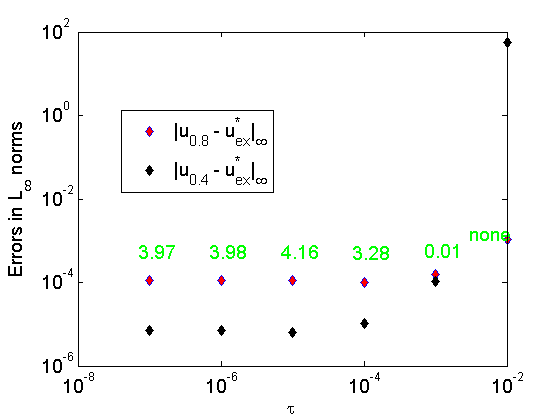
\includegraphics[width=\linewidth]{ConvergenceDecreaseTau.png}
		\centerline{\ref{figConvSeq}a) }
	\end{minipage}	
	\begin{minipage}[b]{0.46\linewidth}
		\raggedright
		 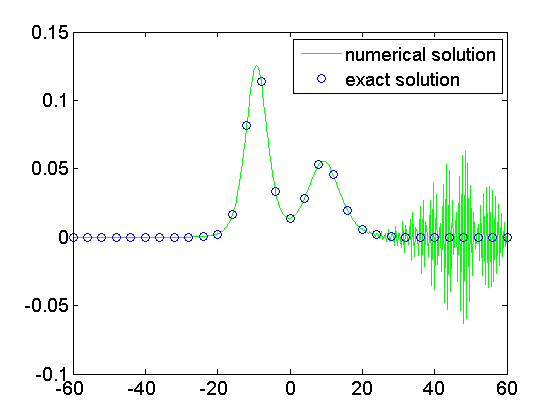
\includegraphics[width=\linewidth]{endSolNumSolDiverg.png}
		\centerline{\ref{figConvSeq}b) }
	\end{minipage}

	\caption{\ref{figConvSeq}a) On the left panel we see the effect of decreasing the time step $\tau$. Errors $E_i$ are measured in $L_\infty$ norms and fourth approximation order ($p=4$). The green values mark the convergence speed, measured with Runge's rule \rf{Runge}, based on the measured errors $E_i$. 
\ref{figConvSeq}b) On the right panel, the solution diverges as the time step is not small enough. This is numerical example, using the TS approach, with $h=0.4$, $\tau = 0.01$ and end time $T=7$.}
	\label{figConvSeq}
\end{figure}

%\begin{figure}[ht]\vspace{0.2cm}
  %\centering
 % 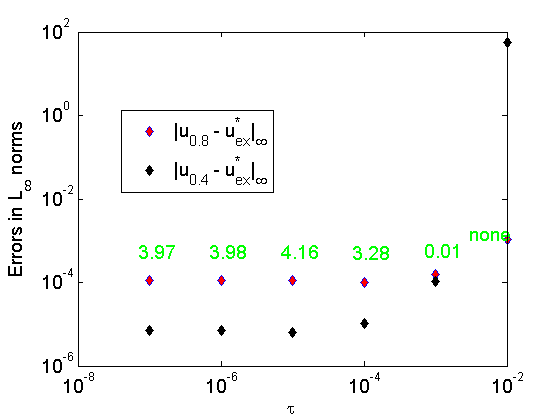
\includegraphics[width=0.5\linewidth]{ConvergenceDecreaseTau.png}
%\caption{On the left panel we see the effect of decreasing the time step $\tau$. Errors $E_i$ are measured in $L_\infty$ norms and fourth approximation order ($p=4$). The green values mark the convergence speed, measured with Runge's rule \rf{Runge}, based on the measured errors $E_i$. On the right panel the solution diverges as the time step is bigger than $h$ squared $\tau > h^2$.}
%\label{figConvSeq}
%\end{figure}
Figure \ref{figConvSeq} shows the effect of modifing the time step $\tau$ on the solution convergence. The nested space grids obtain the following step sizes: $h=0.8, 0.4$, with end time $T=10$. For $\tau>1e-4$, the stability of the Taylor Series method breaks as the $L_2$ and $L_\infty$ errors become much higher compared to the maximum of the solution wave $|u_h|_\infty$. The solution diverges and becomes non-smooth (e.g. the graph is jagged) and there is no convergence. On the other hand, if the step decreases and $\tau<1e-5$, convergence speed is near 4 which reflects the fourth approximation order that is used. The respective convergence speeds and results when using the $L_2$ error norms are similar and are omitted.

\subsection{Numerical Results for the Mass}
The mass is compared on six different grids with space and time steps defined in Table \rf{gridsT}. It is computed using the soluitons from Conservative FDS and Taylor method. For the cases with 
$p=2$, we use Trapezoidal rule for integration. In case of $p=4$ and Taylor method, we use Simpson (1/3) rule. The results are displayed in Table \rf{tableMass}. The first column shows the method which is used. The second column displays the grid variant that is used (see table \rf{gridsT}). The next three columns display the initial mass value $I_0$, maximum deviation above $I_0$ and maximum deviation below $I_0$.
%D
\begin{table}[ht]
\centering
\small
		\begin{tabular}{||c|l|l|l|l||}
			\hline
method        & grid variant ($h,\tau$)& $I_0$ &   $max(I-I_0)$ & $min(I-I_0)$  \\
   			\hline 
Cons FDS            &  1a (0.4, 2.5e-4) & 1.666666e+00 &  4.948717e-09 & -1.959443e-07                    \\
 Taylor               &  1a (0.4, 2.5e-4) & 1.666666e+00 &  4.659617e-08 & 0.000000e+00                \\
Cons FDS            &  1b (0.2, 2.5e-4) & 1.666666e+00 & 3.963669e-10 & -3.424187e-07             \\
 Taylor               &  1b (0.2, 2.5e-4) & 1.666666e+00 & 3.499779e-08 & -1.063058e-09               \\
	   		\hline
			\hline
Cons FDS             & 2a (0.4, 1.0e-6) & 1.666666e+00 & 4.960991e-09 & -4.339504e-08                    \\
 Taylor                & 2a (0.4, 1.0e-6) & 1.666666e+00 & 4.708513e-08 & 0.000000e+00                   \\
Cons FDS            & 2b (0.2, 1.0e-6) & 1.666666e+00 & 3.831861e-10 & -6.643357e-08                  \\
 Taylor                & 2b (0.2, 1.0e-6) & 1.666666e+00 & 2.260040e-08 & -9.728958e-09                      \\
	   		\hline
			\hline
Cons FDS           &  3a (0.8, 6.25e-5) & 1.666667e+00 & 8.198307e-07 & 0.000000e+00                    \\
Taylor                &  3a (0.8, 6.25e-5) & 1.666666e+00 &  3.720412e-08 & 0.000000e+00                      \\
Cons FDS           &  3b (0.4, 6.25e-5) & 1.666667e+00 &  2.714807e-06 & -5.367586e-09                     \\
Taylor                &  3b (0.4, 6.25e-5) & 1.666666e+00 &  3.002585e-08 & -2.842618e-09                      \\
			\hline 
			\hline
		\end{tabular}
		\caption{ The mass and its deviations from initial value measured on different grids. }
\label{tableMass}
\end{table}
One could see that all deviations are lower (at least 10 times) than the errors measured when comparing the numerical solution with the exact one (see Table \rf{tableC} and Table \rf{tableA}). On Figure \rf{massFig} one could see the mass plotted for Grid 1. The values of the mass for Grid 2 and 3 are similar and thus are omitted. Table \rf{tableMass} and Figure \rf{massFig} confirm that the mass is constant over a fixed interval time ([0, 10]).

\begin{figure}[ht]\vspace{0.2cm}
  \centering
  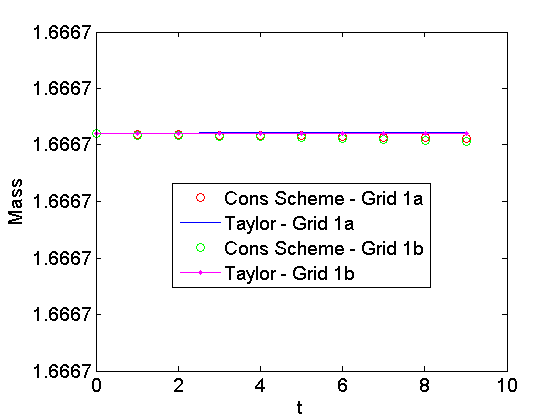
\includegraphics[width=0.5\linewidth]{mass.png}
\caption{The mass of the solution on Grid 1, using the solutions from both Conservative FDS and Taylor method.}
\label{massFig}
\end{figure}

\subsection{Numerical Results for the shape of the solution}

The following paragraph discusses the shape of the solution obtained by the Conservative FDS and Taylor method. Both methods are benchmarked on six different grids with space and time steps defined in Table \rf{gridsT}.

Thus, the Conservative scheme produces six numerical solutions with second approximation order over the grids in Table \rf{gridsT}, while the Taylor method uses second approximation order on Grid 1 and fourth on Grid 2 and Grid 3. The numerical solutions that were obtained for the measurement of the convergence speed in Table \rf{tableA}, are also used here in Table \rf{compareTable}. The end time is $T=10$ and the boundaries of the space domain are $L_1 = L_2 = 60$.

\begin{table}[ht]
\centering
\small
		\begin{tabular}{|c|l|l|l|l|l|l|l|}
			\hline
           Grid                    & Variant   &    $|u_{ex}-u_{T}|_{L2}$  &    $|u_{ex}-u_{C}|_{L2}$  &   $|u_{ex}-u_T|_{\infty}$ &   $|u_{ex}-u_C|_{\infty}$   &  $|u_{ex}|_{\infty}$      \\
			\hline
           Grid 1          &     a:  $h=0.4$  &  $ 7.669196e-04$       &     $7.904798e-04$               &     $5.838980e-04$           &               $6.023530e-04$     &       $1.279362e-01$ \\
			\hline
           Grid 1          &     b:  $h=0.2$  &  $ 1.200402e-04$       &     $1.353479e-04$               &     $1.274495e-04$           &               $1.451817e-04$     &       $1.281769e-01$ \\
			\hline
           Grid 2          &     b:  $h=0.4$  &  $ 9.118794e-06$       &     $1.636122e-03$               &     $7.064211e-06$           &               $1.067977e-03$     &       $1.279362e-01$ \\
			\hline
           Grid 2          &     b:  $h=0.2$  &  $ 3.715136e-07$       &     $ 1.506615e-04$               &     $3.563062e-07$           &               $1.587225e-04$     &       $1.281769e-01$ \\
			\hline
           Grid 3          &     b:  $h=0.8$  &  $ 1.962184e-04$       &     $ 4.630863e-03$               &     $1.058293e-04$           &               $2.537092e-03$     &       $1.278007e-01$ \\
			\hline
           Grid 3          &     b:  $h=0.4$  &  $ 1.044382e-05$       &     $  7.955113e-04$               &     $ 6.808462e-06$           &               $6.066573e-04$     &       $1.279362e-01$ \\
			\hline
		\end{tabular}
	\caption{ Comparison of the Taylor method  $u_{T}$ and the Conservative FDS $u_{C}$ with the exact solution $u_{ex}$.}
	\label{compareTable}
\end{table}

Table \rf{compareTable} compares the numerical solutions from the Taylor method and the Conservative FDS with the exact formula \rf{orgBsqSol}. The first two columns define the type of used grid. The next two columns show the errors of both methods in $L_2$ norms and the next two - errors in $L_\infty$ norms. The last column displays the maximum of the soluiton (at $T=10$) on the used grid. Decreasing the time or space steps leads to smaller errors
for both methods. For the Grid 1 we used only second approximation order $p=2$ and thus the errors for both methods are similar. Nevertheless for Grid 2 and Grid 3 the Taylor method uses fourth approximation order whereas 
the Conservative FDS uses only second. Thus, the errors measured with the Taylor method are at least $151$ times (or much) smaller on Grid 2 and at least $23$ times (or much) smaller on Grid 3 when compared to the errors from the Conservative FDS. In conclusion, the Taylor method produces finer results with smaller error when $p=4$. Nevertheless, the Conservative FDS is between 100 and 1000 times faster when using bigger time steps $\tau < h^2$ which is not possibible in the case of the Taylor method with $p=4$ because of stability restrictions (see Figure \rf{figConvSeq}).

\subsection{Numerical Results for the shape of the solution and its mass and energy on a longer time interval $T = 35$}

Here, we present results for a longer time interval $[0, 35]$, obtained using the Conservative FDS and Taylor method. On Figure \rf{sol35} one could see the evolution of the shape for that time, using the Conservative FDS. An analogous picture is obtained for the Taylor method and is omitted. The results discussed below are summarized in Table \rf{final35}. 

\begin{figure}[H]\vspace{0.2cm}
	\centering
	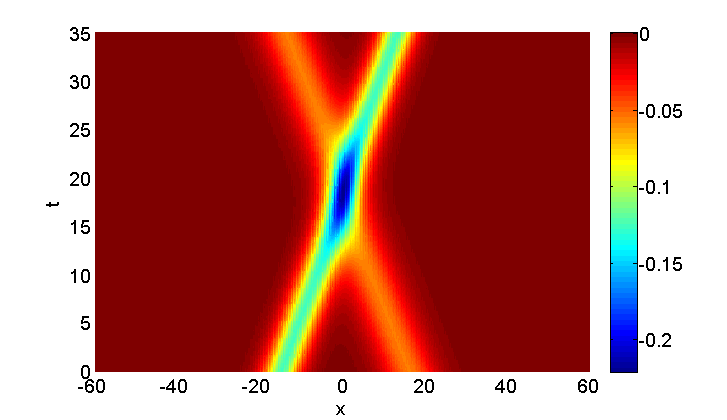
\includegraphics[width=0.7\linewidth]{solution2.png}
\caption{Evolution of the shape over a larger time interval $[0, 35]$. The soluiton is produced using the Conservative FDS.}
\label{sol35}
\end{figure}
The errors measured in $L_2$ and $L_\infty$ norms for the Conservative FDS are $0.001257$ and $0.000640$. The space and time steps are as follow: $h = 0.4$ and  $\tau = 0.05$, with $\sigma = 0.75$. The initial energy equals $0.89$ and its maximum deviation from the initial value equals $1.4076e-04$. The initial mass equals $1.66$ and its maximum deviation from the initial value equals $2.3608e-04$.

The errors measured in $L_2$ and $L_\infty$ norms for the Taylor method are $0.000629$ and $0.000385$. The space and time steps are as follow: $h = 0.4$ and  $\tau = 0.001$. The initial mass equals $1.66$ and its maximum deviation from the initial value equals $1.1196e-05$.



\begin{table}[ht]
\centering
\small
		\begin{tabular}{|c|l|l|l|l|l|l|}
			\hline
Method                    & $(h, \tau)$   &    $|u_{ex}-u_{h}|_{L2}$  &    $|u_{ex}-u_{h}|_{\infty}$  &   $|E_{h}-E_0|_{\infty}$ &   $|M_{h}-M_0|_{\infty}$       \\
			\hline
           Cons FDS          &  $(0.4,0.05)$  &  $ 0.001207$       &     $0.000640$               &     $1.4076e-04$           &               $2.3608e-04$     \\
			\hline
           Taylor, $p=4$       & $(0.4,0.001)$  &  $0.000629$     &      $0.000385$               &            ---           &               $1.1196e-05$     \\
			\hline
  		\end{tabular}
	\caption{Error norms of the solution, energy (in case of Conservative FDS) and mass. Here $u_{ex}$ is the exact solution \rf{orgBsqSol} and $u_{h}$ is the numerical solution obtained either with the Conservative FDS or with the Taylor method, which is defined in the first column.}
	\label{final35}
\end{table}

At the final moment, the difference between the exact and numerical solutions, measured in $L_2$ and $L_\infty$ norms, is at least 100 times less than the maximum of the wave $|u_h|_\infty = 0.1248$. For that longer time period, the energy and mass norms are also preserved with high accuracy.

\section{Conclusion}

\begin{thebibliography}{99} \normalsize

\bibitem{ref0} Boussinesq, J.V., Theorie des ondes et des remous qui se propagent le long d'un canal rectangulaire horizontal, en communiquant au liquide contenu dans ce canal des vitesses sensiblement pareilles de la surface au fond.  {\it Journal de Mathematiques Pures et Appliquees}, \textbf{17} (1872), 55-108.

\bibitem{ref21} Chertok, A., Christov, C.I., Kurganov, A., Central-Upwind Schemes for the Boussinesq Paradigm Equations,
{\it Computational Science and High Performance Computing IV, Notes Numer. Fluid Mech.}, \textbf{113} (2011), 267-281.

\bibitem{ref1} Christov, C.I., An energy-consistent dispersive shallow-water model,  {\it Wave Motion}, \textbf{34} (2001), 161-174.

\bibitem{samarski} Samarskii, A., The Theory of Difference Schemes, Marcel Dekker Inc., New York, 2001.

\bibitem{refHyp} Angelow K., Comparison between two numerical methods for solution of 2D Boussinesq paradigm equation, \emph{AIP Conference Proceedings}, \textbf{2522}, (2022), 090001

\bibitem{consCitat} Kolkovska N., Dimova M., A new conservative finite difference scheme for Boussinesq Paradigm equation, \emph{ Central European Journal of Mathematics}, \textbf{10} (2012), 3

\bibitem{exactSol1} A.-M. Wazwaz. Multiple-soliton solutions for the Boussinesq equation. \emph{Applied Mathematics and Computation}, \textbf{192(2)} (2007), 479–486
\bibitem{exactSol2} N. Fenyvesi and G. Bene. Collision of water wave solitons., \emph{Cent. Eur. J. Phys.}, textbf{11(11)} (2013), 1605–1615

\end{thebibliography}
\end{document}





